\documentclass[unicode,12pt,aspectratio=169,dvipdfmx]{beamer}
\usepackage{bxdpx-beamer}
\usetheme[progressbar=frametitle]{metropolis}
\renewcommand{\kanjifamilydefault}{\gtdefault}
\usepackage{bm}
\usepackage{minted}


\title{\textbf{研究進捗報告}}
\author{竹本志恩}
\date{\today}

\begin{document}

% Slide 1: Title
\begin{frame}
  \titlepage
\end{frame}

% Slide 3: 研究背景
\section{研究背景}
\begin{frame}{これまでの研究背景}
    \begin{itemize}
        \item 少子高齢化による介護負担の増大
        \begin{itemize}
            \item 高齢者が増加
            \item 出生率低下で労働人口が減少
            \item 成り手減少で介護人材が不足
            \item 今後増える見込みはなく,負担軽減策が必要
        \end{itemize}
        \item 安価で手軽な見守りシステムの需要
        \begin{itemize}
            \item 介護業務を一部自動化
            \item 迅速な対応
            \item 監視の負担軽減
        \end{itemize}
    \end{itemize}
\end{frame}

\begin{frame}{研究背景に対する疑問}
  \begin{itemize}
    \item 施設での運用で介護者の負担は減る?
    \begin{itemize}
        \item 本当にそれがやりたいことなのか?
    \end{itemize}
    \item 「安価+手軽さ」だけで、既存の技術と差別化できる?
    \begin{itemize}
        \item 他のセンサー(カメラ、ウェアラブル等)と比較して本当に手軽?
        \item なぜ「音」を選ぶのか、理由が必要
    \end{itemize}
    \item なぜ機械学習を用いる?
    \begin{itemize}
        \item HAR(Human Activity Recognition)には、より古典的で、適用範囲は狭いが確実性の高い手法も存在するのでは?
    \end{itemize}
  \end{itemize}
\end{frame}


\begin{frame}{研究背景を再考}
    以下を念頭に置き,より深掘り
    \begin{itemize}
        \item \textbf{AAL (Ambient Assisted Living)}を汲む
        \begin{itemize}
            \item 自立した生活を支援
            \item 在宅での介護/医療を視野に
            \begin{itemize}
                \item 施設より在宅の方が自立に近づく
                \item 問題の早期発見で医療/介護負担を軽減
                \item 費用や労働量など,高齢者とサービス提供者の負担を軽減
            \end{itemize}
        \end{itemize}
    \item \textbf{音特有の異常行動兆候の探求}
        \begin{itemize}
            \item 音独自の健康指標に着目
            \item 呼吸音や咳き込みなど
        \end{itemize}
    \end{itemize}
\end{frame}


\begin{frame}{研究背景を再考}
  \begin{itemize}
    \item \textbf{機械学習を用いる理由}
    \begin{itemize}
        \item 環境への適応
        \begin{itemize}
            \item 従来法は閾値で判断; 適応的な手法も存在
            \item 機械学習は柔軟で多様な環境に適応可能
        \end{itemize}
        \item \textbf{在宅見守りへの応用}
        \begin{itemize}
            \item 支援があれば自立生活が可能な高齢者を対象に考える
            \item 単一目的の検知より,様々な異常の兆候を柔軟に検知したい
        \end{itemize}
    \end{itemize}
  \end{itemize}
\end{frame}

% Slide 4: 全体ロードマップ
\section{研究計画}
\begin{frame}{仮ロードマップ}
  \begin{itemize}
    \item 今後2週間で計画を具体化
    \item \textbf{7月: 基礎の準備}
    \begin{itemize}
        \item 背景サーベイ
        \item マルチラベル音響イベント検知モデルの実装
        \item データ収集
    \end{itemize}
    \item \textbf{8月: 必要な施策の実行}
    \begin{itemize}
        \item 半教師あり連合学習の調査・実装
        \item シミュレーション方法の調査・検討
    \end{itemize}
    \item \textbf{9月: 異常検知層の追加}
    \item \textbf{10月: FLの実装・実験}

  \end{itemize}
\end{frame}

% Slide 5: 今後の実験評価計画
\begin{frame}{具体化のための計画}
  \begin{itemize}
    \item 以下を検証し,研究計画の目処を付ける
    \item \textbf{主要タスク}
    \begin{itemize}
        \item $\checkmark$基礎モデル構築
        \item データ収集
        \item データ不均衡対策
        \item 半教師あり連合学習
        \item 異常検知モデルの構築
        \item シミュレーションの検討
    \end{itemize}
  \end{itemize}
\end{frame}

% Slide 6: 現在の進捗
\section{現在の進捗}
\begin{frame}[fragile]{実装: マルチラベル音響検知モデル (PoC)}
  \begin{itemize}
    \item \textbf{モデル:} CNN $\rightarrow$Transformerベース
    \item \textbf{データ生成:}
    \begin{itemize}
        \item ESC-50データセットの一部カテゴリを使用
        \item 2つの音の組み合わせを全パターン作成 (約12,000)
        \item ラベルの組が均衡になるよう9,048データを選定
    \end{itemize}
    \item 使用ラベルは雨やドアのノック音など(cf. 補足)
    \item 日常生活の基本的な音を想定
  \end{itemize}
\end{frame}

% Slide 7: モデル定義
% \begin{frame}{実装: モデル定義}
%   \begin{itemize}
%     \item 先輩の実装を参考に、Transformerベースのモデルを実装中
%   \end{itemize}
%     \textbf{モデル構造の概要}
%     \begin{enumerate}
%       \item Input (Batch, Freq, Time)
%       \item BatchNorm1d
%       \item Permute
%       \item Linear (Embedding)
%       \item \textbf{Encoder} (PositionalEncoding + N × EncoderBlock)
%       \begin{itemize}
%           \item EncoderBlock: Multi-Head Attention, FeedForward Network
%       \end{itemize}
%       \item Permute
%       \item AdaptiveAvgPool1d
%       \item Classifier (Linear)
%       \item Sigmoid (Multi-label Output)
%     \end{enumerate}
% \end{frame}

% Slide 8: 学習と評価
\begin{frame}[fragile]{実装: 学習と評価}
    \begin{columns}[T]
        \begin{column}{0.5\textwidth}
            \textbf{学習}
            \begin{itemize}
                \item 選択した9,048データで訓練
                \item パラメータなど: 補足へ
                \item マルチラベル用の構成
\begin{minted}[fontsize=\small]{bash}
* 出力: Sigmoid関数
* 最適化アルゴリズム: Adam
* 損失関数: バイナリクロスエントロピー
\end{minted}
            \end{itemize}
        \end{column}
        \begin{column}{0.5\textwidth}
            \textbf{評価}
            \begin{itemize}
                \item 訓練時と異なる936データを使用
                \item 各精度指標
\begin{minted}[fontsize=\small]{bash}
Micro Precision/Recall/F1 
= 0.9655 / 0.8682 / 0.9143
Macro   F1 = 0.8458
\end{minted}
            \end{itemize}
        \end{column}
    \end{columns}
\end{frame}

% Slide 9: 研究目的の再考
\begin{frame}{サーベイ: 研究背景の再考}
  \begin{itemize}
    \item \textbf{現状の反省:} 技術ありきで話を進めており、研究意義の説明が不足
    \item \textbf{対応:}
    \begin{itemize}
        \item 関連論文を読み、研究背景を深掘り中
        \item サーベイ論文を3本程度確認済み
        \item 今後、サーベイ論文から引用されている重要論文を精読予定
    \end{itemize}
  \end{itemize}
\end{frame}

% Slide 10: データ収集
\begin{frame}{データ収集: 異常イベントの音響データ}
  \begin{itemize}
    \item 音特有の異常(呼吸、咳き込み、悲鳴など)に関するデータを収集したい
    \item \textbf{調査済みデータセット}
    \begin{itemize}
        \item \textbf{Deeply Nonverbal Vocalization Dataset}: 作者への連絡が必要
        \item \textbf{Respiratory Sound Database}:
        \begin{itemize}
            \item デジタル聴診器の音源が多く、行動認識には不向きか
            \item `AKG C417L Microphone`の音源は使える可能性あり
            \item ライセンスが不明
        \end{itemize}
    \end{itemize}
    \item \textbf{未確認データセット候補}
    \begin{itemize}
        \item \textbf{SAFE}: 転倒音
        \item \textbf{TAME Pain Dataset}: 痛みに関連する音声
        \item \textbf{Sound-Dr Dataset}: おそらく呼吸音
        \item \textbf{F2LCough}: 咳の分類
    \end{itemize}
  \end{itemize}
\end{frame}

% Slide 11: 今後のステップと課題
\section{展望と課題}
\begin{frame}{今後の展望}
    \begin{itemize}
        \item \textbf{各種対応の簡易的な試行} (所要時間とタスク内容の把握)
        \begin{itemize}
            \item \textbf{データ不均衡対応:} Focal Lossなどの導入を検討
            \item \textbf{半教師あり連合学習}の調査,検証
            \item \textbf{異常検知モデル}の構築
            \item \textbf{シミュレーション}環境の検討
        \end{itemize}
        \item \textbf{AALサーベイの継続}
        \begin{itemize}
            \item 類似研究を調査し、研究の新規性・貢献を明確に
        \end{itemize}
        \item \textbf{データ収集と分析}
        \begin{itemize}
            \item 各種データセットの内容を精査
            \item 音で検知可能な異常の兆候を洗い出す
        \end{itemize}
    \end{itemize}
\end{frame}

\begin{frame}{課題}
    \begin{itemize}
        \item \textbf{懸念事項: 自作データセットの評価方法}
        \begin{itemize}
            \item 構築したデータセットでモデルをどう評価する?
            \item どうすれば実用に耐えうるモデルだと示せるか
            \item マルチラベルデータ作成時,現実的なラベル設計が重要そう
        \end{itemize}
    \end{itemize}
\end{frame}


\section{補足}

\begin{frame}[fragile]{補足: 使用ラベル}
    \begin{itemize}
        \item \textbf{使用ラベル (ESC-50より抜粋)}
\begin{minted}[fontsize=\small]{python}
allowed_categories = [
    "rain", "door_wood_knock", "door_wood_creaks", 
    "glass_breaking", "sneezing", "breathing", "coughing",
    "footsteps", "laughing", "brushing_teeth", "snoring", 
    "drinking_sipping", "pouring_water", "toilet_flush"
]
    \end{minted}
    \end{itemize}
\end{frame}


\begin{frame}[fragile]{補足: 学習と評価}
    \begin{columns}[T]
        \begin{column}{0.5\textwidth}
            \textbf{学習のHyperparameters:}
\begin{minted}[fontsize=\scriptsize]{python}
model = MelSpectrogramTransformer(
    input_dim=n_mels,
    embed_dim=128,      # 埋込次元
    nhead=4,            # Attnヘッド数
    nhid=256,           # FFN隠れ層
    nlayers=2,          # Encoder層数
    n_classes=num_classes,
    max_len=X.shape[2])
\end{minted}
            \textbf{実行コマンド例:}
\begin{minted}[fontsize=\scriptsize]{bash}
uv run model_module/train.py \
     --data ./dataset/esc50_multilabel.npz \
     --batch 32 \
     --epochs 20 \
     --lr 1e-3 \
     --val-split 0.1 \
     --device cuda \
     --save-model ./checkpoints/label-14_transformer.pth
\end{minted}
        \end{column}
        \begin{column}{0.5\textwidth}
            \textbf{評価}
             \textbf{実行コマンド例:}
\begin{minted}[fontsize=\scriptsize]{bash}
uv run ./model_module/eval.py \
  --data    ./dataset/esc50_multilabel.npz \
  --model   ./checkpoints/label-14_transformer.pth \
  --batch   64 \
  --device  mps \
  --threshold 0.5

  [RESULT]
Threshold = 0.50
Micro Precision/Recall/F1 
= 0.9655 / 0.8682 / 0.9143
Macro   F1                = 0.8458

\end{minted}
        \end{column}
    \end{columns}
\end{frame}

\begin{frame}[fragile]{補足: Classification Report (per class):}
\begin{minted}[fontsize=\scriptsize]{bash}
                        precision    recall  f1-score   support
            Class rain       0.94      0.84      0.89        19
 Class door_wood_knock       1.00      0.85      0.92        20
Class door_wood_creaks       1.00      0.83      0.91        18
  Class glass_breaking       1.00      0.80      0.89        20
        Class sneezing       0.89      0.85      0.87        20
       Class breathing       1.00      0.55      0.71        20
        Class coughing       0.89      0.96      0.92        25
       Class footsteps       1.00      0.93      0.97        15
        Class laughing       1.00      0.88      0.93        16
  Class brushing teeth       1.00      1.00      1.00        25
         Class snoring       0.95      0.95      0.95        19
Class drinking_sipping       0.96      0.88      0.92        25
   Class pouring_water       1.00      0.94      0.97        16
    Class toilet_flush       0.00      0.00      0.00         0

             micro avg       0.97      0.87      0.91       258
             macro avg       0.90      0.80      0.85       258
          weighted avg       0.97      0.87      0.91       258
           samples avg       0.98      0.87      0.90       258
\end{minted}
\end{frame}


\begin{frame}{補足: 研究背景}
    \begin{itemize}
    \item サーベイ前に書いた研究背景
    \item 今後サーベイを通じて詰める
    \end{itemize}
 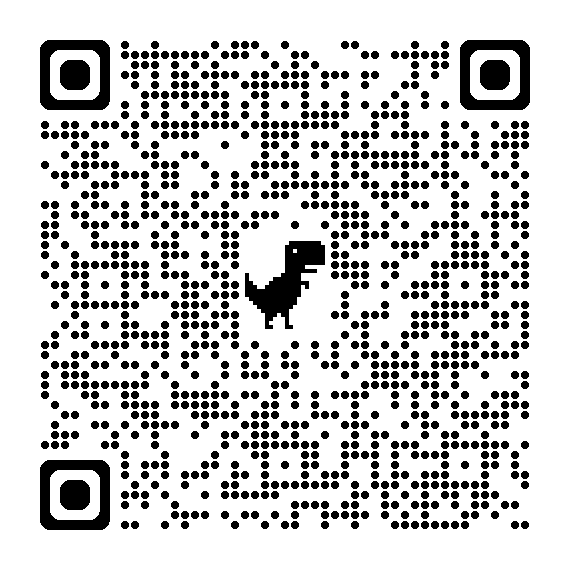
\includegraphics[width=5cm]{figures/qrcode_scrapbox.io.png}
\end{frame}


\end{document}